\name{c vs. s Decision Problem}
Decide whether  $ \dps\OPT(I) \geq c $ or  $ \OPT(I)<s $. If  $ \OPT(I) \geq c $, return YES, else if $ \OPT(I)<s $, return NO.

\name{c vs. s Decision Problem}
Given  $ I  $ \st  $ \OPT(I) \geq c $, find a solution  $ x $  \st  $ \mathrm{Val}(x;I) \geq s $.

\begin{theorem}
    Suppose  $ A  $ solves  c vs. s Search problem in poly-time, then  $ \exists  $ poly-time  $ A' $ that solves c vs. s decision problem.   
\end{theorem}
The algorithm is as follows:
\begin{algorithm}[H]
    \caption{c vs. s Search}
    \begin{algorithmic}[1]
        \STATE $ x\leftarrow A(I) $
        \IF{ $ \mathrm{Val}(x;I) \geq s $ }
        \STATE return YES
        \ELSE
        \STATE return NO
        \ENDIF
    \end{algorithmic}
\end{algorithm}

\begin{fact}
    \,
    \begin{enumerate}[label=(\arabic*)]
        \item  $ A  $ is  $ \alpha $-approximation algorithm  $ \Rightarrow  $  $ A  $ is  $ c $ vs.  $ \alpha c $ search algorithm  $ \forall c $.
        \item  $ \exists  $  $ c $ vs.  $ s(c)  $ search algorithm  $ \Rightarrow   $ $ \exists  $ $ \alpha $-approximation algorithm where  $ \alpha=\dps\inf_c\{\frac{s(c)}{c}\} $
        \item (contrapositive of  $ A $ )  $ c $ vs.  $ s $ decision problem "hard"  $ \Rightarrow  $  $ \frac{s}{c} $-approximation algorithm "hard".           
    \end{enumerate}
\end{fact}
\begin{remark}
    The same  $ c $ vs.  $ s $ algorithm in max-cut and min-uncut problems might correspond to quite different approximation ratios.  
\end{remark}
\subsection{Set-Cover}
\begin{example}[Set-Cover]
    Universe  $ U=\{1,2,\cdots,n\} $.  $ S_1,S_2,\cdots,S_M\subset U $.
    
    Our goal is to find  $ T\subset\{S_1,\cdots, S_M\} $ such that  $ \dps\cup_{S\in T }S=U $ and  $ |T| $ minimized.  
\end{example}

Of course, it can be represented as \textbf{Max-Coverage} problem: Given additional input  $ k $. Find  $ T\subset\{S_1,\cdots, S_M\} $ \st  $ |T|=k $ and  $ |\dps\cup_{S\in T }S| $ maximized.

It has a greedy algorithm:
\begin{algorithm}[H]
    \caption{Greedy}
    \begin{algorithmic}[1]
        \STATE $ T\leftarrow\emptyset $ 
        \REPEAT
            \STATE Let  $ S_i $ be the set that covers the most uncovered elements.
            \STATE  $ T\leftarrow T\cup\{S_i\} $.
            \STATE  $ U\leftarrow U\setminus S_i $.
        \UNTIL  $ \begin{cases}
            \text{All elements covered}&\text{set cover}\\
            |T|=k&\text{max-coverage}
        \end{cases} $    
    \end{algorithmic}
\end{algorithm}
\begin{fact}
    Suppose  $ \exists  $  $ m $ sets covering  $ U $. After  $ t $ choices,  $ T $ covers    $ \dps 1-\left(1-\frac{1}{m}\right)^t $ fraction of elements.
\end{fact}
\begin{corollary}
    The greedy algorithm is  $ \lceil \ln n\rceil  $ approximation for set-cover 
\end{corollary}
\begin{proof}
    Let  $ m=\OPT $. After  $ t=\lceil \ln n\rceil \cdot m$ choices, number of uncovered elements 
    \[\left(1-\frac{1}{m}\right)^{\lceil \ln n\rceil \cdot m}\cdot n \geq \frac{1}{n}=1\]
\end{proof}
\begin{corollary}
    Greedy is  $ 1 $ vs.  $ 1-\frac{1}{e} $ approximation for Max-coverage.  
\end{corollary}
\begin{proof}
    Set  $ m=k $. After  $ t=k $ choices, coverage of  $ T $: 
    \[1-(1-\frac{1}{k})^k \geq 1-\frac{1}{e}\]   
\end{proof}
\begin{fact}
    1 vs. 1- $ \gamma $ approximation for ma-coverage  $ \Rightarrow  $  $ \lceil \log_{1-\gamma}\frac{1}{n}\rceil $-approximation for set-cover. 
\end{fact}
\begin{proof}
    "Guess"  $ k=\OPT^{\mathrm{set-cover}} $.
    
    Repeatly invoke  $ A(k)\cdot\lceil \log_{1-\gamma}\frac{1}{n}\rceil $ times. Then number of uncovered elements 
    \[n\cdot(1-\gamma)^{\lceil \log_{1-\gamma}\frac{1}{n}\rceil} \geq n\cdot \frac{1}{n}=1\]
\end{proof}
In fact, we can construct  an extreme case for greedy algorithm:

\begin{figure}[htbp]
    \centering
    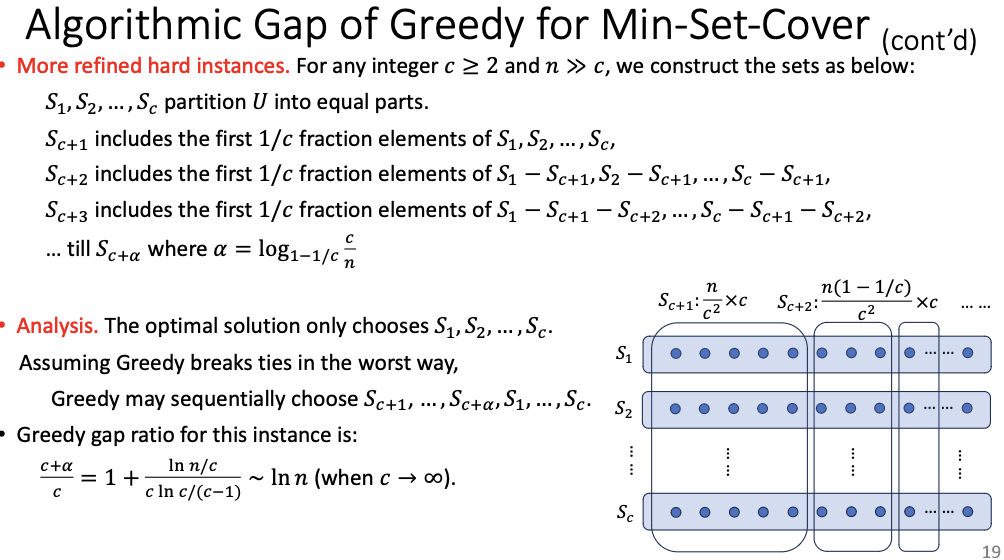
\includegraphics[width=\textwidth]{D11-set_cover_extreme_case.png}
    \caption{Extreme case for greedy algorithm}
\end{figure}
\subsection{Weighted Min Set-cover}
\begin{example}[Weighted Min Set-cover]
    Given  $ n $ elements,  $ M $ sets,  $ S_1,\cdots,S_M\subset U $. Each set  $ S_i $ has a weight  $ w(S_i)>0 $.

    Now select  $ T\subset\{S_1,\cdots, S_M\} $ such that  $ \dps\sum_{S\in T}w(S) $ minimized. 
\end{example}
Integer Program: Minimize  $ \dps\sum_{i=1}^M w(S_i)x_i $. Subject to   $ \dps\sum_{i:j\in S_i} x_i \geq 1$,  $ \forall j\in U $, where  $ x_i\in \{0,1\} $,  $ \forall i\in [M] $.

If we relax the integer constraint, we have an LP relaxation:  $ x_i\in[0,1] $, which can be solved in poly-time since it is a linear program.

We need "rounding" to transform fractional solution to the integer solution.

\subsubsection{Randomized Rounding}
If  $ \{x_i^*\} $ is the optimal LP solution.  For each  $ s_i $, select  $ s_i\in T $ independently with probability   $ \min\{\alpha x_i^*,1\} $. Then 
\[\Ebb[w(T)] \leq \alpha\sum_{i=1}^M w(s_i),\,x_i^*=\alpha\cdot \mathrm{LP} \leq \alpha\cdot \mathrm{OPT}\] 

Now we want to estimate  $ \mathrm{Pr}[T\text{ covers }U] $.

If there is some  $ \alpha x_i^ \geq 1 $, then  $ \mathrm{Pr}(T\text{ covers }U)=1 $. If  $ \forall i, x_i^*<1 $,   
then 
\[\begin{aligned}
    \mathrm{Pr}[T\text{ covers }U]&=1-\mathrm{Pr}[ \exists j\in U , j\not\in T ]\\
    & \geq 1-\sum_{j\in U}\mathrm{Pr}[j\not\in T]\\
    &=1-\sum_{j\in U}\prod_{i: j\in S_i}(1-\min\{\alpha x_i^*,1\})\\
    & \geq 1-\sum_{j\in U}\prod_{i: j\in S_i}\exp(-\alpha x_i^*)\qquad\text{(If some $ x_i^*<1 $, the probability will be 0)}\\
    &=1-\sum_{j\in U}\exp(-\sum_{j\in S_i}\alpha x_i^*)\\
    &=1-\sum_{j\in U}\exp(-\alpha)
\end{aligned}\]

Therefore, we obtain 
\begin{claim}
    \[\mathrm{Pr}(\text{every element covered}) \geq 1-n\cdot e^{-\alpha}\]
\end{claim}
If we set  $ \alpha=\ln n+\ln\ln n $, then 
\begin{align*}
    \mathrm{Pr}[\epsilon_1]\mathrm{Pr}[\text{every element covered}]&\geq 1-n\cdot e^{-\ln n-\ln\ln n}\\
    &=1-\frac{1}{n\ln n}\\
    &\geq 1-\frac{1}{\ln n}
\end{align*} 
We should also focus on  $ \Ebb(w(T)) \leq \alpha\cdot\OPT $. Here we use the \name{Markov Inquality}:
\begin{theorem}[Markov Inequality]
    For Random Variable  $ X \geq 0 $,  $ \mathrm{Pr}(X \geq t\mathbb EX) \leq \frac{1}{t} $  
\end{theorem} 
\begin{proof}
    \begin{align*}
        \Ebb X&=\Ebb[X|X \geq \alpha]\cdot \mathrm{Pr}(X \geq \alpha)+ \Ebb[X|X < \alpha]\cdot \mathrm{Pr}(X < \alpha)\\
        & \geq \alpha\cdot\mathrm{Pr}[X \geq \alpha]
    \end{align*}
    Therefore,  $ \mathrm{Pr}[X \geq \alpha] \leq \frac{\Ebb X}{\alpha} $ 
\end{proof}
So 
\begin{align*}
    \mathrm{Pr}[\epsilon_2]\mathrm{Pr}\left[\sum_{i}w(S_i)y_i\geq (\ln n+2\ln\ln n)\OPT\right]& \leq \frac{\ln n+\ln\ln n}{\ln n+2\ln \ln n} \\
    &=1-\frac{\ln \ln n}{\ln n+2\ln\ln n}
\end{align*}
So the union probablity 
\[\begin{aligned}
    \mathrm{Pr}[\epsilon\wedge \bar{\epsilon}_2]& \geq \mathrm{Pr}[\epsilon_1]-\mathrm{Pr}[\epsilon_2]\\
    & \geq \frac{\ln\ln n}{\ln n+2\ln\ln n}-\frac{1}{\ln n}\\
    & \geq \Omega(\frac{\ln\ln n}{\ln n})\xrightarrow{\text{boost}}1-\frac{1}{n^{100}}
\end{aligned}\]

\begin{theorem}
    With probability  $ \Omega(\frac{\ln\ln n}{\ln n}) $, LP+randomized rounding returns a  $ (\ln n+2\ln \ln n) $-approximation solution.  
\end{theorem}

The question is how to boost the probability. Indeed, if we independently round  $ N  $ times, 
\begin{align*}
    \mathrm{Pr}[\exists 1\text{ trial succeeds}]& \geq 1-[1-\Omega(\frac{\ln\ln n}{\ln n})]^N\\
    & \geq 1-\exp(-\Omega(\frac{\ln\ln n}{\ln n}\cdot N))\\
    & \geq 1-\exp(-\Omega(n\cdot\ln n)) \geq 1-e^{-n}
\end{align*}
if we set  $ N\leftarrow (\ln n)\cdot n $ in the last step.

Apply the method to Max-coverage problem, Integer Problem is to  $\max \dps\sum_{j=1}^n$ such that 
\begin{align*}
    \sum_{i=1}^M x_i &\leq k\\
    y_j& \leq \sum_{j\in S_i}x_i,\forall j\in [n]\\
    y_j& \leq 1,\forall j\in [n]\\
    x_i&\in\{0,1\},\forall i\in [M]
\end{align*} 
So the LP relaxation is to relax  $ x_i\in [0,1] $. 

Repeat  $ k  $ times and select set  $ i  $ with probability  $ \dps\frac{x_i^*}{k} $.

\begin{align*}
    \Ebb[\text{coverges}]& =\sum_{j=1}^n\mathrm{Pr}[j\text{ covered}]\\
    &=\sum_{j=1}^n\left(1-\left(1-\sum_{j\in S_i}\frac{x_i^*}{k}\right)^k\right)\\
    & \geq \sum_{j=1}^n\left(1-\exp(-\sum_{j\in S_i}x_i^*)\right)\\
    & \geq \sum_{j=1}^n\left(1-\exp(-y_i^*)\right)\\
    & \geq \alpha\sum_{j=1}^n y_j^*=\alpha\cdot \mathrm{LP} \geq \alpha\cdot \OPT
\end{align*}
where  $ \alpha=1-\frac{1}{e} $ 

The estimation is tight for this rounding if we consider the set  $ \mathcal{U}=\{0,1\}^k $ and  $ S_{i,0}=\{a\in U|a_i=0\} $,  $ S_{i,1}=\{a\in U|a_i=1\} $.   


\subsubsection{Integrality Gap}
Instance  $ I  $ is a  $ c $ vs.  $ s $-\name{Integrality Gap (IG) instance} if  $ \mathrm{LP}(I) \geq c $ and  $ \OPT(I) \leq s $. The \name{gap ratio} is  $\dps \frac{c}{s} $. 

\begin{enumerate}
    \item Large IG $ \Rightarrow  $ Inaccurate estimation of LP.
    \item The estimation of rounding algorithm is usually 
    \[\mathrm{rounding } \geq \cdots \geq \alpha\cdot\mathrm{LP} \geq \alpha\cdot\OPT\]
    Since  $ \mathrm{rounding} \leq \OPT $ in maximization problem, if IG is large,  $ \alpha $ can be very large and hence the approximation ratio is very bad. 
\end{enumerate}

For instance, consider the set-cover problem that is to minimize  $ \dps\sum_{i=1}^M x_i $ \st 
\[\sum_{j\in S_i}x_i \geq 1,\forall j\in U,\quad x_i\in [\{0,1\},\forall i\in [M]]\] 
relax the condition  $ x_i\in [0,1] $ and consider the set  $ \mathcal{U}=\{0,1\}^q\setminus\{0\} $ and  $ S_{\vec{\alpha}}=\{l\in U:l^T\alpha=1\pmod 2\} $ for  $ \alpha\in \{0,1\}^q $ with the size  $  M=2^q,n=2^q-1 $. 

\[|S_{\vec{\alpha}}|=\begin{cases}
    2^{q-1}&\alpha\neq 0\\
    0&\alpha=0
\end{cases}\]

\begin{claim}
    LP=2
\end{claim}
\begin{proof}
    Take  $ x_{\vec{\alpha}}=\frac{2}{2^q} $. Then  $ \dps\sum_{\vec{\alpha}}S_{\vec{\alpha}}=2 $. And the LP constraint met where
    \[\forall \vec{e}\in U,\,\sum_{\vec{e}\in S_{\vec{\alpha}}}\frac{2}{2^q}=2\mathrm{Pr}_{\vec{\alpha}\in \{0,1\}^q}[\vec{e}\in S_{\vec{\alpha}}]=2\times \frac{1}{2}=1\] 
    
    Certainly  $ \mathrm{LP} \geq 2 $, so  $ \mathrm{LP}=2 $.  
\end{proof}

But we also have a claim about  $ \OPT $:

\begin{claim}
     $ \OPT \geq q $. So the instance is a  $ 2 $ vs.  $ q $ IG with ratio  $ \frac{q}{2}=\frac{1}{2}\log_2(n+1)=\frac{\ln(n+1)}{2\ln 2} $.   
\end{claim}
\begin{proof}
    For any  $ S_{\vec{\alpha}_1},\cdots,S_{\vec{\alpha}_{q-1}} $, suppose  $ S_{\vec{\alpha}_1}\cup\cdots\cup S_{\vec{\alpha}_{q-1}} $ is a cover of  $ U $. Then 
    \begin{align*}
        &\Leftrightarrow \bar{S}_{\vec{\alpha}_1}\cap\cdots\cap\bar{S}_{\vec{\alpha}_{q-1}}=\{\vec{0}\}\\
        &\Leftrightarrow\{\vec{e}\in \{0,1\}^q:e^T\vec{\alpha}_i=0\forall i\in [q-1]\}=\{\vec{0}\}
    \end{align*} 
    which is impossible!
\end{proof}